\documentclass[a4paper,11pt,dvipdfmx]{jsarticle}


% 数式
\usepackage{amsmath,amsfonts}
\usepackage{bm}

% 画像
\usepackage[dvipdfmx]{graphicx}
\usepackage{framed}

% 図形
\usepackage{tikz}
\usepackage{circuitikz}
\usepackage[utf8]{inputenc}
\usepackage{geometry}
\geometry{margin=2cm}
\usetikzlibrary{shapes.geometric}
\usetikzlibrary {shapes.misc}

% ソースコード
\usepackage{listings,jlisting,color}
\lstset{
basicstyle={\ttfamily},
identifierstyle={\small},
commentstyle={\smallitshape},
keywordstyle={\small\bfseries},
ndkeywordstyle={\small},
stringstyle={\small\ttfamily},
frame={tb},
breaklines=true,
columns=[l]{fullflexible},
numbers=left,
xrightmargin=0zw,
xleftmargin=3zw,
numberstyle={\scriptsize},
stepnumber=1,
numbersep=1zw,
lineskip=-0.5ex
}
\renewcommand{\lstlistingname}{ソースコード}

\usepackage{booktabs}

\usepackage{pgfplots}
\pgfplotsset{compat=1.18} % 最新の互換性を指定


\begin{document}
\definecolor{shadecolor}{gray}{0.70}

\begin{titlepage}
\noindent
\vspace{4cm}
\begin{center}
\begin{LARGE}
組込システムI \\
第8回  課題 \\
\vspace{8cm}
提出日  2025/06/12 \\
学籍番号  21T2166D \\
名前  渡辺 大樹 \\
\end{LARGE}
\end{center}
\end{titlepage}
\setcounter{page}{1}

\section{課題}
本課題では、Raspberry Piと4桁7セグメントLED、BCD-to-7セグメントデコーダIC(74HC4511)を用いて、デジタル時計およびカレンダー表示システムを実装する。具体的には、演習(2)として以下の機能を実現する:
\begin{enumerate}
    \item Raspberry Piのシステム時刻を取得し、4桁7セグメントLEDに表示する。
    \item 表示モードは「時・分(HHMM)」と「月・日(MMDD)」の2種類とする。
    \item タクトスイッチを押すことで、表示モードを切り替える。
    \item 時刻および日付の十の位が0の場合は、その桁をブランク(非表示)にする。例えば、8時5分は「 8 05」、3月5日は「 3 05」のように表示する。
\end{enumerate}
本課題を通じて、7セグメントLEDのダイナミック点灯(マルチプレキシング)の原理、BCDデコーダICの利用方法、イベント駆動によるスイッチ入力処理、およびPythonのdatetimeモジュールを用いた時刻情報の扱について理解を深めることを目的とする。

\section{使用部品}
本演習で使用した主な部品は以下の通りである。
\begin{itemize}
    \item Raspberry Pi 4B
    \item 4桁7セグメントLED(カソードコモン、例:OptoSupply OSL40562-LR)
    \item BCD-to-7セグメントデコーダIC(74HC4511)
    \item タクトスイッチ(1個)
    \item 抵抗:1k$\Omega$(7個、セグメント電流制限用、74HC4511の出力とLEDセグメント間。ただし、スライドの回路図には1k$\Omega$とあるが、74HC4511の出力電流能力とLEDの仕様に応じて適切な値を選定する。今回はスライドの指示に従う。)
    \item ブレッドボード
    \item ジャンパー線
\end{itemize}

\section{回路の説明}
本システムでは、Raspberry PiのGPIOピンを使用して、74HC4511デコーダIC、4桁7セグメントLED、およびタクトスイッチを制御する。

\textbf{使用したRaspberry PiのGPIOピン(BCM番号と物理ピン番号):}
\begin{itemize}
    \item BCDデータ出力 (74HC4511へ):
    \begin{itemize}
        \item GPIO20 (Pin 38) - D0
        \item GPIO21 (Pin 40) - D1
        \item GPIO22 (Pin 15) - D2
        \item GPIO23 (Pin 16) - D3
    \end{itemize}
    \item 7セグメントLED 桁選択 (カソード制御):
    \begin{itemize}
        \item GPIO24 (Pin 18) - DIG1
        \item GPIO25 (Pin 22) - DIG2
        \item GPIO26 (Pin 37) - DIG3
        \item GPIO27 (Pin 13) - DIG4
    \end{itemize}
    \item スイッチ入力:
    \begin{itemize}
        \item GPIO16 (Pin 36) - Switch
    \end{itemize}
    \item 電源:
    \begin{itemize}
        \item +3.3V (Pin 1 or Pin 17)
        \item GND (Pin 39 or others)
    \end{itemize}
\end{itemize}

\textbf{回路構成:}
\begin{itemize}
    \item Raspberry PiのGPIO20-GPIO23を74HC4511のBCD入力D0-D3に接続する。
    \item 74HC4511のセグメント出力a-gを、それぞれ1k$\Omega$の電流制限抵抗を介して4桁7セグメントLEDの対応するセグメント入力に接続する。
    \item 74HC4511の制御ピンは、LT (Lamp Test) と BL (Blanking) を+3.3Vに、LE (Latch Enable) をGNDに接続し、トランスペアレントモードで動作させる。VCCは+3.3V、GNDはGNDに接続する。
    \item Raspberry PiのGPIO24-GPIO27を4桁7セグメントLEDの各桁のコモンカソード(DIG1-DIG4)に接続する。これにより、特定の桁をLOWにすることでその桁を点灯させる。
    \item タクトスイッチの一端をRaspberry PiのGPIO16に、もう一端を+3.3Vに接続する。GPIO16は内部プルダウン抵抗を有効にして使用する。
\end{itemize}

\section{回路図}
\begin{figure}[htbp]
\centering
\begin{circuitikz}[american, scale=0.9, every node/.style={scale=0.8}]
    % Raspberry Pi 4B representation
    \draw[thick] (0,0) rectangle (3,8);
    \node at (1.5,8.5) {\textbf{Raspberry Pi 4B}};

    % RPi Pins
    \node[anchor=east] at (0,7.5) {Pin 1}; \node[anchor=west] at (0.2,7.5) {+3.3V};
    \node[anchor=east] at (0,7) {Pin 38 (GPIO20)}; \node[anchor=west] at (0.2,7) {D0};
    \node[anchor=east] at (0,6.5) {Pin 40 (GPIO21)}; \node[anchor=west] at (0.2,6.5) {D1};
    \node[anchor=east] at (0,6) {Pin 15 (GPIO22)}; \node[anchor=west] at (0.2,6) {D2};
    \node[anchor=east] at (0,5.5) {Pin 16 (GPIO23)}; \node[anchor=west] at (0.2,5.5) {D3};
    \node[anchor=east] at (0,5) {Pin 18 (GPIO24)}; \node[anchor=west] at (0.2,5) {DIG1};
    \node[anchor=east] at (0,4.5) {Pin 22 (GPIO25)}; \node[anchor=west] at (0.2,4.5) {DIG2};
    \node[anchor=east] at (0,4) {Pin 37 (GPIO26)}; \node[anchor=west] at (0.2,4) {DIG3};
    \node[anchor=east] at (0,3.5) {Pin 13 (GPIO27)}; \node[anchor=west] at (0.2,3.5) {DIG4};
    \node[anchor=east] at (0,1) {Pin 36 (GPIO16)}; \node[anchor=west] at (0.2,1) {SW};
    \node[anchor=east] at (0,0.5) {Pin 39}; \node[anchor=west] at (0.2,0.5) {GND};

    % Power lines
    \draw[red, thick] (3,7.5) -- (14,7.5) node[above,pos=0.5] {+3.3V}; % VCC rail
    \draw[black, thick] (3,0.5) -- (14,0.5) node[below,pos=0.5] {GND}; % GND rail

    % Switch
    \draw (3,1) -- (14,1) to[push button, l=SW] (14,7.5); % Switch to 3.3V

    % 74HC4511
    \draw (5,3) rectangle (8,7);
    \node at (6.5,7.2) {74HC4511};
    % Inputs D0-D3
    \draw (3,7) -- (5,6.2); \node[anchor=west] at (5,6.2) {D0(7)};
    \draw (3,6.5) -- (5,5.8); \node[anchor=west] at (5,5.8) {D1(1)};
    \draw (3,6) -- (5,5.4); \node[anchor=west] at (5,5.4) {D2(2)};
    \draw (3,5.5) -- (5,5); \node[anchor=west] at (5,5) {D3(6)};
    % Control Pins LE, BL, LT
    \draw (5,4.6) node[anchor=west] {LE(5)} -- (4,4.6) -- (4,0.5); % LE to GND
    \draw (5,4.2) node[anchor=west] {BL(4)} -- (4.5,4.2); % BL to VCC
    \draw (5,3.8) node[anchor=west] {LT(3)} -- (4.5,3.8) -- (4.5,7.5); % LT to VCC
    % Power for 74HC4511
    \draw (5,3.4) node[anchor=west] {GND(8)} -- (4,3.4); % GND
    \draw (8,6.4) node[anchor=east] {VCC(16)} -- (8.5,6.4) -- (8.5,7.5); % VCC

    % Segment outputs a-g (with resistors)
    \coordinate (s_a) at (8,6); \node[anchor=east] at (s_a) {a(13)};
    \coordinate (s_b) at (8,5.6); \node[anchor=east] at (s_b) {b(12)};
    \coordinate (s_c) at (8,5.2); \node[anchor=east] at (s_c) {c(11)};
    \coordinate (s_d) at (8,4.8); \node[anchor=east] at (s_d) {d(10)};
    \coordinate (s_e) at (8,4.4); \node[anchor=east] at (s_e) {e(9)};
    \coordinate (s_f) at (8,4); \node[anchor=east] at (s_f) {f(15)};
    \coordinate (s_g) at (8,3.6); \node[anchor=east] at (s_g) {g(14)};

    % 4-Digit 7-Segment LED (Cathode Common)
    % Represent as a block
    \draw[thick] (10,2) rectangle (13,7);
    \node at (11.5,7.3) {4-Digit 7-Seg LED};
    \node at (11.5,1.7) {(Cathode Common)};

    \node[anchor=north] at (9,6.8) {1k$\Omega$};
    % Segment inputs to LED (shared)
    \foreach \y/\name/\labelpos in {6.5/a/s_a, 6/b/s_b, 5.5/c/s_c, 5/d/s_d, 4.5/e/s_e, 4/f/s_f, 3.5/g/s_g} {
        \draw (\labelpos) -- ++(0.5,0) to[R] ++(1,0) -- (10,\y);
        \node[anchor=west] at (10,\y) {\name};
    }
    % Digit select (common cathodes)
    \draw (3,5) -- (3.5,5) -- (3.5,2.8) -- (10,2.8); \node[anchor=west] at (10,2.8) {DIG1};
    \draw (3,4.5) -- (3.6,4.5) -- (3.6,2.6) -- (10,2.6); \node[anchor=west] at (10,2.6) {DIG2};
    \draw (3,4) -- (3.7,4) -- (3.7,2.4) -- (10,2.4); \node[anchor=west] at (10,2.4) {DIG3};
    \draw (3,3.5) -- (3.8,3.5) -- (3.8,2.2) -- (10,2.2); \node[anchor=west] at (10,2.2) {DIG4};
    % Common cathodes are pulled to GND by RPi GPIOs to light up.
\end{circuitikz}
\caption{演習(2)の回路図}
\label{fig:circuit_exam8}
\end{figure}

\section{アルゴリズムの説明}
本システムの制御はPythonスクリプト(`exam8-2.py`)によって行われる。アルゴリズムの主要な部分は以下の通りである。

\begin{enumerate}
    \item \textbf{初期設定 (`setup`関数):}
    \begin{itemize}
        \item GPIOのモードをBCMに設定。
        \item BCD出力ピン (D0-D3) を出力モードに設定。
        \item 桁選択ピン (DIG1-DIG4) を出力モードに設定し、初期状態をHIGH(全桁非表示)にする。カソードコモンなのでLOWで点灯。
        \item スイッチ入力ピン (PIN\_SWITCH) を入力モードに設定し、内部プルダウン抵抗を有効にする。
        \item スイッチ入力ピンに立ち上がりエッジ検出のイベントを設定し、コールバック関数 `switch\_callback` を登録する。チャタリング防止のため、`bouncetime`を300msに設定。
    \end{itemize}

    \item \textbf{スイッチ処理 (`switch\_callback`関数):}
    \begin{itemize}
        \item スイッチが押されるたびにグローバル変数 `display\_mode` の値を 'time' と 'date' の間でトグルする。
    \end{itemize}

    \item \textbf{BCDデータ送信 (`send\_to\_bcd`関数):}
    \begin{itemize}
        \item 表示したい数字(0-9)を引数として受け取る。
        \item 事前に定義されたBCDコードの辞書 `BCD\_CODES` を参照し、対応する4ビットのBCDデータを取得する。
        \item 0-9以外の数字(特に、先頭の0を消すために使用する15)が指定された場合は、全ビットが1のコード(通常はブランク表示)を出力する。
        \item 取得したBCDデータをGPIOピン (D0-D3) に出力する。
    \end{itemize}

    \item \textbf{表示ループ (`display\_loop`関数):}
    \begin{itemize}
        \item 無限ループで以下の処理を繰り返す(ダイナミック点灯)。
        \item 現在の日時を `datetime.datetime.now()` で取得する。
        \item `display\_mode` の値に応じて、表示する4つの数字(時・分または月・日)をリスト `display\_digits` に格納する。
        \item 時・分表示の場合:`[時(十の位), 時(一の位), 分(十の位), 分(一の位)]`
        \item 月・日表示の場合:`[月(十の位), 月(一の位), 日(十の位), 日(一の位)]`
        \item 各ペア(時、分、月、日)の十の位が0の場合、その桁をブランク表示にするため、対応する `display\_digits` の要素を15に置き換える。
        \item 4つの桁を順番に高速に切り替えて点灯させる(ダイナミック点灯)。
        \begin{enumerate}
            \item 全ての桁選択ピンをHIGHにして全桁を消灯する。
            \item 表示する桁の数字に対応するBCDデータを `send\_to\_bcd` 関数で74HC4511に送信する。
            \item 対応する桁選択ピンをLOWにしてその桁を点灯させる。
            \item 短時間 (0.002秒) 待機する。この遅延がダイナミック点灯の周期を決定する。
        \end{enumerate}
    \end{itemize}
    \item \textbf{メイン処理 (`main`関数):}
    \begin{itemize}
        \item `setup`関数を呼び出して初期化を行う。
        \item `display\_loop`関数を呼び出して表示を開始する。
        \item `KeyboardInterrupt` (Ctrl+C) を検出するとプログラムを終了し、`GPIO.cleanup()` でGPIO設定を解放する。
    \end{itemize}
\end{enumerate}
このアルゴリズムにより、少ないGPIOピンで4桁の数字を表示し、スイッチ入力で表示内容を切り替えるシステムが実現される。

\section{結果}
本課題で実装したシステムは、設計通りに動作することを確認した。\\
また実験した際のRaspberry Piの本体時刻は`print(datetime.datetime.now())`より`2025-05-09 18:22:25.162019`と確認できた  
\begin{enumerate}
    \item 電源投入後、4桁7セグメントLEDには現在の時刻が「HHMM」形式で「18 21」と表示された。
    \item タクトスイッチを押すと、表示が現在の月日に「MMDD」形式で切り替わり「 5  9」と表示された。
    \item 再度タクトスイッチを押すと、表示は時刻表示に戻った。この切り替え動作はスイッチを押すたびに繰り返された。
    \item ダイナミック点灯により、4つの桁が連続的に点灯しているように見え、チラツキも許容範囲内であった。`time.sleep(0.002)` の設定により、各桁の点灯時間は2msとなり、全体のフレームレートは約125Hz ($1 / (4 \times 0.002\text{s})$) となるため、人間の目にはほぼ連続点灯として認識された。
    \item スイッチのチャタリングは `bouncetime=300ms` の設定により効果的に防止され、一度の押下で確実に表示モードが切り替わった。
\end{enumerate}
以下に、実際にブレッドボード上に組んだ回路の写真を示す(図\ref{fig:circuit_photo_exam8})。
\begin{figure}[htbp]
\centering
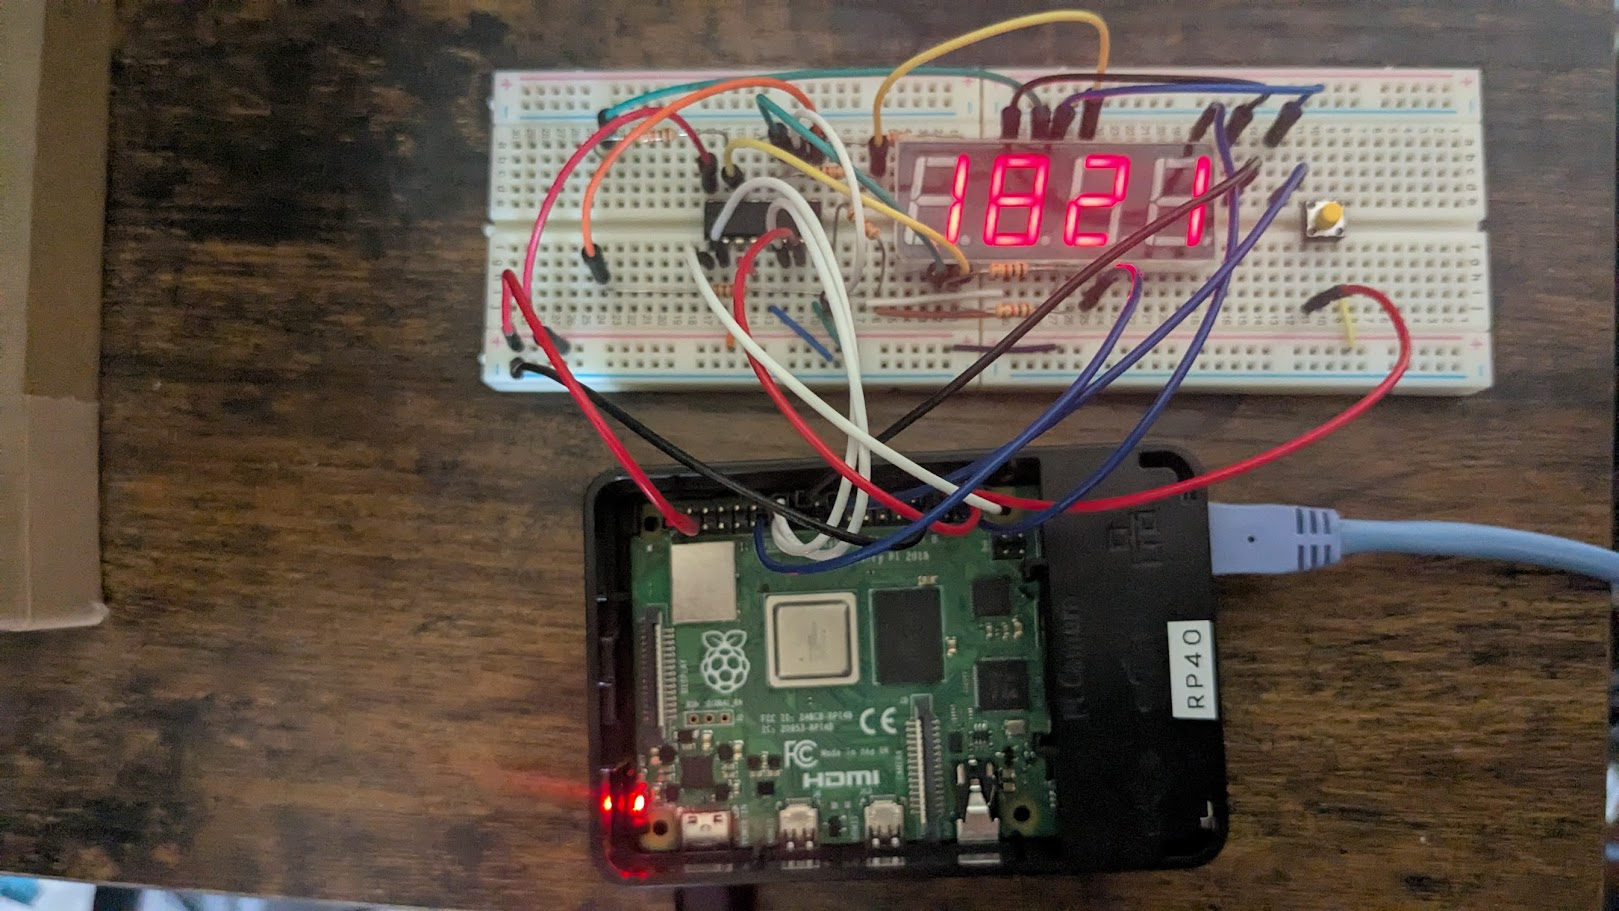
\includegraphics[width=0.8\textwidth]{image.png}
\caption{実装した回路の写真}
\label{fig:circuit_photo_exam8}
\end{figure}
写真では、Raspberry Pi、ブレッドボード、7セグメントLED、74HC4511 IC、タクトスイッチ、および配線が確認できる。LEDには時刻または日付が意図した通りに表示された。

\section{考察}
本演習を通じて、以下の点について理解を深めることができた。
\begin{itemize}
    \item \textbf{ダイナミック点灯の有効性:} 4桁の7セグメントLEDを駆動するために、セグメント制御用(7本、BCDデコーダ経由なら4本)と桁選択用(4本)のGPIOピンのみで済むため、ピン数の限られたマイクロコントローラにおいて非常に有効な技術である。本演習ではBCDデコーダIC(74HC4511)を使用したため、BCD入力4ピン+桁選択4ピンの計8ピンで4桁の数字を表示できた。ソフトウェアによる高速な切り替えにより、人間の目には全桁が同時に点灯しているように見える残像効果を利用している点を実感した。
    \item \textbf{BCDデコーダICの利便性:} 74HC4511のようなBCD-to-7セグメントデコーダを使用することで、マイクロコントローラ側は表示したい数字のBCDコードを出力するだけで済み、7セグメントの各セグメントを直接制御する複雑なロジックをソフトウェアで実装する必要がなくなる。これにより、CPU負荷の軽減とプログラムの簡略化が図れる。
    \item \textbf{イベント駆動処理:} スイッチ入力の処理に `GPIO.add\_event\_detect` を用いたイベント駆動方式を採用することで、CPUが常にスイッチの状態をポーリングする必要がなくなり、リソースを効率的に使用できる。コールバック関数により、スイッチが押された瞬間にのみ対応する処理が実行されるため、応答性も向上する。
    \item \textbf{datetimeモジュールの活用:} Pythonの `datetime` モジュールを使用することで、現在時刻や日付の取得、およびそれらの要素(時、分、月、日)へのアクセスが容易に行えることを確認した。
    \item \textbf{表示の工夫:} 時刻や日付の十の位が0の場合にブランク表示にする処理は、ユーザーインターフェースの観点から視認性を高める効果がある。74HC4511ではBCDコード10〜15がブランク表示となる特性を利用してこれを実現した。
    \item \textbf{回路設計の注意点:} 7セグメントLEDの各セグメントには適切な電流制限抵抗を接続することが重要である。また、74HC4511の制御ピン(LE, BL, LT)の処理(プルアップ/プルダウン)もICの仕様に従って正しく行う必要がある。今回はLEをGNDに接続してトランスペアレントモードとした。
\end{itemize}
今後の改善点としては、表示のチラツキをさらに低減するためのリフレッシュレートの最適化や、より多くの情報を表示するための工夫(例えばドットマトリクスLEDの使用)などが考えられる。

\section{問いの解答}
\textbf{問い:4桁LEDがアノードコモンであった場合、今回の演習はどの様な構成とすれば良いか。}

\textbf{解答:}
4桁7セグメントLEDがアノードコモンであった場合、回路構成と制御方法にいくつかの変更が必要となる。主な変更点は以下の通りである。

\begin{enumerate}
    \item \textbf{桁選択(コモンアノード制御):}
    \begin{itemize}
        \item アノードコモンの場合、各桁の共通アノード端子に+3.3V(または適切な駆動電圧)を供給することでその桁がアクティブになる。Raspberry PiのGPIOピンで直接駆動する場合、桁選択ピン(DIG1〜DIG4)はHIGHを出力することで対応する桁を選択(点灯準備)し、LOWで非選択とする。
        \item Pythonコードでは、桁選択部分のロジックが逆になる。初期状態で全桁選択ピンをLOW(非アクティブ)にし、点灯させたい桁のピンをHIGHにする。
        \begin{verbatim}
# 初期化時 (setup関数内)
# GPIO.output(pin, GPIO.HIGH) を GPIO.output(pin, GPIO.LOW) に変更
for pin in DIGIT_PINS:
    GPIO.setup(pin, GPIO.OUT)
    GPIO.output(pin, GPIO.LOW) # 全桁を初期状態で非表示

# 表示ループ内 (display_loop関数内)
# GPIO.output(DIGIT_PINS[i], GPIO.LOW) を GPIO.output(DIGIT_PINS[i], GPIO.HIGH) に変更
GPIO.output(DIGIT_PINS[i], GPIO.HIGH) # 選択した桁を点灯
# 消灯時は GPIO.output(pin, GPIO.HIGH) を GPIO.output(pin, GPIO.LOW) に変更
for pin in DIGIT_PINS:
    GPIO.output(pin, GPIO.LOW) # 全桁を非表示
        \end{verbatim}
        \item GPIOの出力電流能力を超える場合は、PNPトランジスタや専用のドライバIC(例:ULN2003Aの逆の使い方やTD62783Aなど)を介してアノードを駆動する必要がある。
    \end{itemize}

    \item \textbf{セグメント制御:}
    \begin{itemize}
        \item アノードコモンの場合、各セグメント(a〜g)は対応するピンをLOWにすることで点灯する。
        \item 使用している74HC4511は、BCD入力に応じてアクティブHIGH(HIGHでセグメント点灯)の信号をセグメント出力ピンに出力する。これはカソードコモンLEDに適している。
        \item アノードコモンLEDで74HC4511をそのまま使用する場合、74HC4511の各セグメント出力とLEDのセグメント入力の間にNPNトランジスタやインバータIC(例:74HC04)を挟み、信号を反転させる必要がある。
        \item あるいは、アノードコモン用のBCD-to-7セグメントデコーダIC(例:74LS48など、アクティブLOW出力を持つもの)に変更する。この場合、74LS48はTTLレベルなので、Raspberry Piの3.3Vロジックとのレベル変換に注意が必要な場合がある。CD4543Bなどもアノードコモンに対応できる設定がある。
        \item 電流制限抵抗は引き続き各セグメントに必要となる。
    \end{itemize}

    \item \textbf{74HC4511の制御ピン(LE, BL, LT)と電源:}
    \begin{itemize}
        \item これらの制御はLEDの種類(アノードコモン/カソードコモン)に直接依存しないため、変更は不要。VCC, GNDの接続も同様。
    \end{itemize}
\end{enumerate}
まとめると、アノードコモンLEDを使用する場合は、主に桁選択の駆動方法(GPIO出力の論理反転、場合によってはドライバ追加)と、セグメント信号の論理反転(デコーダICの変更または反転回路の追加)が必要となる。ソフトウェア側では、桁選択のGPIO出力論理を反転させる修正が主となる。

\section{付録:ソースコード}
\lstinputlisting[caption=exam8-2.py]{C:/Program_Code/Python/BuiltIn/8/exam8-2.py}

\end{document}
